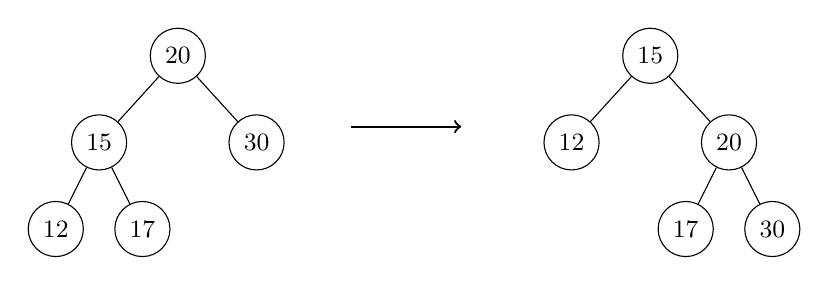
\begin{tikzpicture}[level distance=1.1cm,every node/.style={draw,circle,minimum size=0.7cm,inner sep=1pt,font=\small},
 level 1/.style={sibling distance=2cm},level 2/.style={sibling distance=1.1cm},baseline=(a.base)]
\node (a) at (0,0) {20} child {node {15} child {node {12}} child {node {17}}} child {node {30}};
\draw[->,thick] (2.2,-0.9) -- (3.6,-0.9);
\begin{scope}[xshift=6cm]
\node {15} child {node {12}} child {node {20} child {node {17}} child {node {30}}};
\end{scope}
\end{tikzpicture}
